\section{Realisierung flache FSM}

\subsection{Mögliche Realisierungen von flachen FSMs}

\begin{outline}
    \1 Steuerkonstrukt (typischerweise mit \textbf{switch-case})
        \2 prozedural oder objektorientiert
    \1 Definition und Abarbeitung einer \textbf{Tabelle}
        \2 prozedural oder objektorientiert
    \1 \textbf{State Pattern} (Gang of Four, GoF)
        \2 nur objektorientiert
    \1 Generisch mit Templates
        \2 nur mit einer Sprache, die Templates unterstützt (z.B. C++)
\end{outline}

\vspace{0.2cm}

\textrightarrow\ Alle Varianten haben wie immer sowohl Vor- als auch Nachteile \\
\textrightarrow\ Bei allen Varianten sind auch Variationen vorhanden


\subsection{Realisieurng mit Steuerkonstrukt (prozedural in C)}

\subsubsection{State-Event-Diagram -- Up/Down-Counter}

\begin{center}
    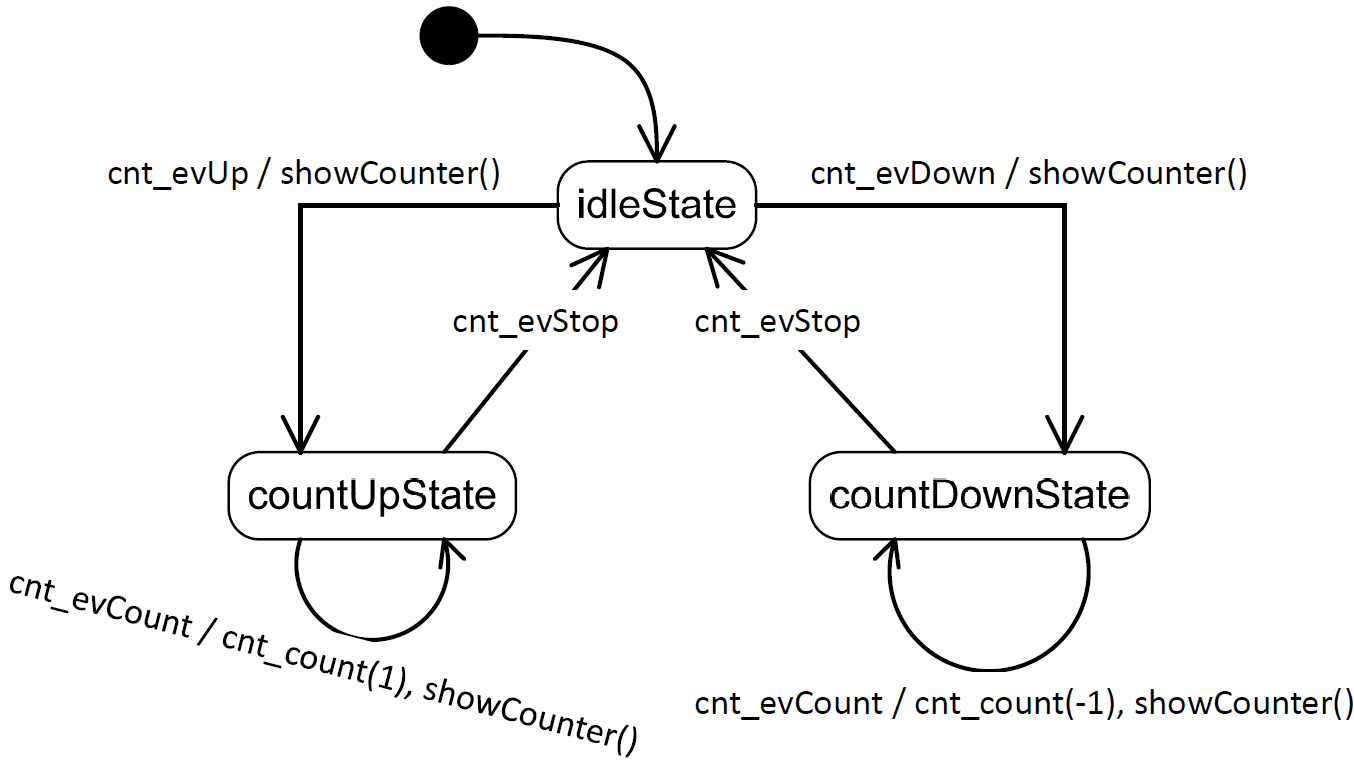
\includegraphics[width=0.7\columnwidth]{images/fsm_up-down-counter_diagramm_C.png}
\end{center}


\subsubsection{Implementation der Prozeduralen Realisierung in C}

\begin{outline}
    \1 \textbf{Ereignisse (events)}
        \2 Schnittstelle nach aussen \textrightarrow\ ändern Zustand der FSM
        \2 In enum definiert (\textbf{public}) \textrightarrow\ header-file
        \2 Einzelne Events und enum Bezeichnung enthalten \textbf{Unitkürzel} (hier: \mylstbox{cnt_})
    \1 \textbf{Zustände (states)}
        \2 In enum definiert (\textbf{nicht} public) \textrightarrow\ sourcecode-file
    \1 \textbf{Aktueller Zustand} wird in einer \textbf{statischen Varianlen} gehalten
    \1 Die FSM wird in \textbf{zwei Funktionen} implementiert
        \2 Initialiserungs-Funktion (hier: \mylstbox{void cnt_ctrlInit(int initValue)})
        \2 Prozess-Funktion (hier: \mylstbox{void cnt_ctrlProcess(cnt_Event e)}) \\
            \textrightarrow\ Zustände prüfen, Zustandsübergänge veranlassen
    \1 Anstossen einer FSM
        \2 Initialisierung in \lstinline|main|-Funktion
        \2 Überprüfung, welches Event aufgetreten ist meist in \mylstbox{do-while}-Schleife
\end{outline}


\subsubsection{Implementation der Prozeduralen Realisierung in C}

\begin{outline}
    \1 Da aktueller Zustand eine statische Variable ist, kann es nur \textbf{eine einzige Instanz} der FSM geben
    \1 Bei mehreren Instanzen in C...
        \2 darf \mylstbox{currentState} nicht \mylstbox{static} sein und muss als Parameter mitgegenen werden,
            bzw. ein Pointer auf die jeweilige Variable
        \2 Zustands-enum muss in die Schnittstelle (header-file) oder es muss z.B. mit \mylstbox{void*} gearbeitet werden
    \1 In C ist \textbf{keine schöne Kapselung} der Attribute möglich (\mylstbox{currentState})
    \1 Funktion \mylstbox{cnt_ctrlProcess()} kann beliebig aufgerufen werden (periodischer Task, laufend, etc.)
    \1 Bei exponierten Funktionen / Definitionen muss in C ein Unitkürzel vorangestellt werden (hier: \mylstbox{cnt_})
\end{outline}


\example{UpD/Down-Counter (prozedural in C)}

% TODO: \para environment not showing...?
% TODO: add keywords an stuff to listings setup

\para{Schnittstelle FSM} 
\lstinputlisting{snippets/fsm_counterCtrl_C.h} 


\para{Implementation FSM} 
\lstinputlisting{snippets/fsm_counterCtrl_C.c}

\para{Anstossen der FSM} 
\lstinputlisting{snippets/fsm_main_counterTest.c}

\columnbreak


\subsection{Realisieurng mit Steuerkonstrukt (objektorientiert in C++)}

% \begin{center}
%     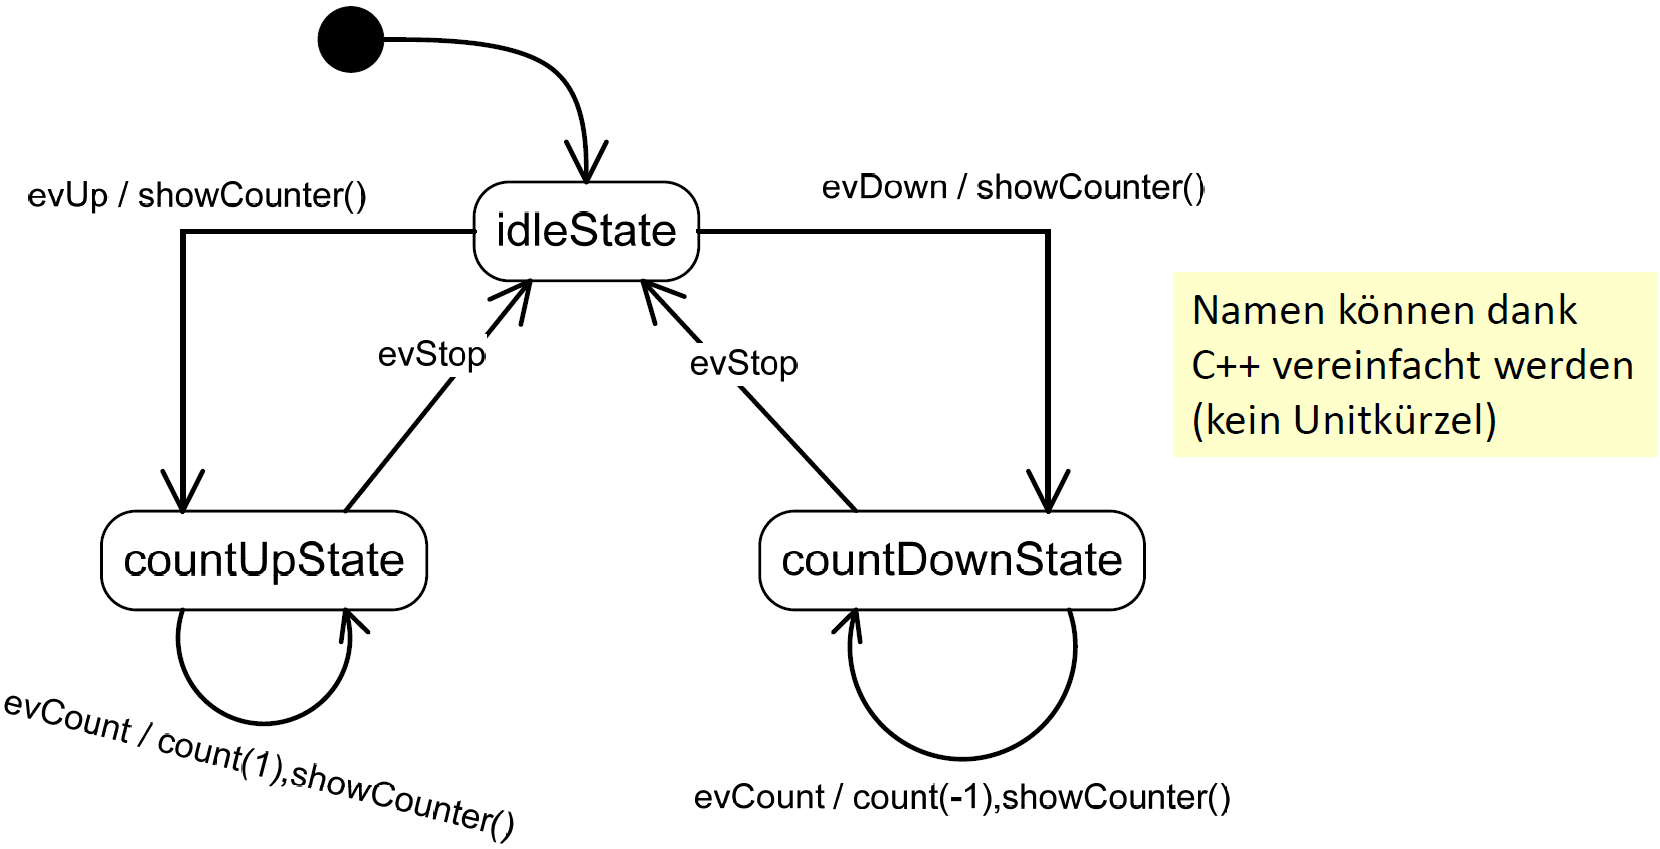
\includegraphics[width=0.7\columnwidth]{images/fsm_up-down-counter_diagramm_CPP.png}
% \end{center}


\subsection{Realisierung mit Tabelle}


\subsubsection{Performancesteigerung mit inline-Funktionen}


\subsubsection{Execution Engine}